\documentclass[11pt,a4paper]{report}
\usepackage[margin=2.5cm]{geometry}
\usepackage{lmodern}
\usepackage[T1]{fontenc}
\usepackage[utf8]{inputenc}
\usepackage{microtype}
\usepackage{booktabs,longtable,array}
\usepackage{graphicx}
\usepackage{xcolor}
\usepackage{listings}
\usepackage{enumitem}
\usepackage{fancyhdr}
\usepackage[colorlinks=true,linkcolor=blue!50!black,urlcolor=blue!50!black,citecolor=blue!50!black]{hyperref}

\newcommand{\ntests}{63}
\newcommand{\npass}{17}
\newcommand{\nxfail}{46}
\newcommand{\nissues}{24}


% ---------- edit these ----------
\newcommand{\studentname}{Your Name}
\newcommand{\studentinst}{Your Institute}
\newcommand{\reportdate}{November 2026}
% --------------------------------

\newcommand{\code}[1]{\texttt{\detokenize{#1}}}
\newcommand{\repo}{\url{https://github.com/osdag-admin/OsdagBridge}}

\lstset{basicstyle=\ttfamily\footnotesize,breaklines=true,frame=single,
        backgroundcolor=\color{black!4},rulecolor=\color{black!25},columns=fullflexible,
        keepspaces=true,showstringspaces=false}

\setlength{\parindent}{0pt}
\setlength{\parskip}{0.55em}
\pagestyle{fancy}\fancyhf{}
\fancyhead[L]{\small OsdagBridge Software Testing \& Issue Reporting}
\fancyhead[R]{\small FOSSEE Winter Internship 2026}
\fancyfoot[C]{\thepage}
\renewcommand{\headrulewidth}{0.3pt}

\begin{document}

% ------------------------------------------------------------------ title
\begin{titlepage}
\centering
\vspace*{1.5cm}
{\Large FOSSEE Winter Internship 2026 --- Screening Task Report}\\[2.2cm]
{\Huge\bfseries OsdagBridge Software Testing \&\\[0.3em] Issue Reporting}\\[1.4cm]
{\large An independent test suite and defect register for\\
the OsdagBridge steel-bridge design software}\\[3cm]
{\large Submitted by}\\[0.4em]
{\Large\bfseries\studentname}\\[0.3em]
{\large\studentinst}\\[2.2cm]
{\large Osdag Project, FOSSEE, IIT Bombay}\\[0.4em]
\reportdate
\vfill
{\small Audited software: OsdagBridge, commit \texttt{2cb7ddc} (7~December~2025)\\
\repo}
\end{titlepage}

% ------------------------------------------------------------------ summary
\chapter*{Summary}
\addcontentsline{toc}{chapter}{Summary}
I tested the OsdagBridge repository from the outside, the way a user or a CI server would: install it,
import it, run its documented commands, and check each promise made in its README. The work produced
\textbf{\ntests{} automated tests} and a register of \textbf{\nissues{} issues}, each with steps to reproduce,
expected and actual behaviour, the test that proves it, and a suggested fix.

\begin{itemize}[leftmargin=1.4em,itemsep=0.2em]
\item \textbf{The package core cannot be imported.} \code{osdagbridge/core/__init__.py} runs
  \code{from .models import *}, but there is no \code{models} module. \textbf{67 of the package's 74 modules fail
  to import} (ISSUE-001, Critical). Removing that one line, or adding an empty file, fixes it.
\item \textbf{The project's own test-suite cannot notice.} All seven upstream test files are \code{assert True}
  placeholders, so \code{pytest} is green while the core is unusable; one file is not even collected
  (ISSUE-023, ISSUE-024).
\item \textbf{A structural check that cannot fail.} \code{check_local_buckling()} takes no inputs and always
  returns \code{True} (ISSUE-014).
\item Of the \nissues{} issues: 1 Critical, 4 High, 9 Medium, 10 Low. Most others are documented features that
  are not implemented yet (CLI, unit conversion, validation, IRC load models).
\end{itemize}

The suite is green today (\npass{} pass, \nxfail{} are \emph{strict expected failures} that each document one
verified defect), and it is built so that fixing a bug turns the matching test red until it is promoted to a
normal regression test.

\tableofcontents

% ------------------------------------------------------------------ 1
\chapter{Introduction}
\section{FOSSEE and the internship}
FOSSEE (Free/Libre and Open Source Software for Education) at IIT Bombay promotes the use of open-source software
in education and offers remote internships in which students contribute to its projects. Applicants complete a
screening task; this report documents my submission for the Osdag project's software-testing task.

\section{Osdag}
Osdag (Open Steel Design and Graphics) is free and open-source software for the design and detailing of steel
structures following the Indian Standard IS~800:2007.

\section{OsdagBridge}
OsdagBridge extends Osdag to bridges. According to its README it is a ``modular, shared-core software plugin for the
analysis and design of steel bridges'': one Python core (\code{osdagbridge.core}) is meant to serve a command-line
interface, a PySide6 desktop application and a Django\,+\,React web application. It lists plate-girder bridges as
supported, three analysis back-ends (a native solver, OpenSeesPy, OspGrillage) and the Indian bridge codes
IRC:6-2017, IRC:22-2015 and IRC:24-2010. Source: \repo.

% ------------------------------------------------------------------ 2
\chapter{Screening Task}
\section{Problem statement}
Test the OsdagBridge software, identify defects, and report them in a form the maintainers can act on:
reproducible steps, expected versus actual behaviour, and severity.

\section{Tasks done}
\begin{enumerate}[leftmargin=1.6em,itemsep=0.15em]
\item Cloned the repository, recorded the audited commit, and installed it into a clean virtual environment.
\item Explored the code and extracted every verifiable promise in the README (install, CLI, desktop, codes, CI,
  paths, examples).
\item Wrote \ntests{} pytest tests in six modules, each probe isolated in its own interpreter.
\item Registered \nissues{} issues in one YAML file and generated the Markdown register and the tables in this report
  from it.
\item Validated the test suite itself (Chapter~\ref{ch:validation}).
\item Added a GitHub Actions workflow and a paced demo script used for the screencast.
\end{enumerate}

% ------------------------------------------------------------------ 3
\chapter{Methodology}
\section{Target and environment}
\begin{center}
\begin{tabular}{@{}ll@{}}
\toprule
Repository & \texttt{osdag-admin/OsdagBridge}\\
Commit & \texttt{2cb7ddc} (``Refactor'', 7 December 2025)\\
Python / pytest & 3.13.18 / 9.1.1\\
Operating system & Linux 6.18, x86\_64\\
Install method & \code{pip install -e .} in a fresh virtual environment\\
\bottomrule
\end{tabular}
\end{center}

\section{Exploration}
The first step was to find out what the software \emph{is}. The repository is an early scaffold: most modules are a
docstring marked ``(stub)'' and one to six lines of code. Installation succeeds, so I walked every module in the
installed package and tried to import it, then ran each command in the README, then compared README claims with the file
tree. Every mismatch became a candidate test.

\section{Design principles}
\begin{description}[leftmargin=1.4em,style=nextline,itemsep=0.3em]
\item[Isolated probes.] ISSUE-001 is an import-time failure. In-process, it would break every later test, so each
  probe runs in a fresh \code{python -I} subprocess with only the tree under test on \code{sys.path}.
\item[Strict expected failures.] A known defect is marked \code{xfail(strict=True, raises=AssertionError)}. The suite
  stays green, but the moment someone fixes the bug the test \emph{unexpectedly passes} and the build fails, which forces
  the test to be promoted to a regression test. \code{raises=AssertionError} means a test cannot be ``expected to fail''
  by crashing for an unrelated reason.
\item[Isolating the blocker.] A \code{patched_src} fixture copies the source tree and adds an empty
  \code{core/models.py}. It lets the suite test the behaviour of everything \emph{behind} ISSUE-001 without hiding
  ISSUE-001 itself. The upstream repository is never modified.
\item[Traceability.] A test cites each finding by ID; \code{test_06_traceability.py} fails if a test cites an unregistered
  issue or an issue has no test, so tests and register cannot drift apart.
\end{description}

\section{Severity scale}
\begin{description}[leftmargin=1.4em,itemsep=0.1em]
\item[Critical] the package cannot be used.
\item[High] a promised feature is absent, or a check gives false assurance.
\item[Medium] documented behaviour does not work.
\item[Low] metadata, documentation or hygiene.
\end{description}

\section{Suite structure}
\begin{center}\begin{tabular}{@{}lrrr@{}}
\toprule
\textbf{Module} & \textbf{Tests} & \textbf{Pass} & \textbf{Documented defect (xfail)}\\
\midrule
Imports & 4 & 2 & 2 \\
CLI / entry points & 8 & 1 & 7 \\
Packaging & 7 & 0 & 7 \\
Core behaviour & 28 & 8 & 20 \\
Docs / repo promises & 13 & 3 & 10 \\
Traceability & 3 & 3 & 0 \\
\midrule
\textbf{Total} & \textbf{63} & \textbf{17} & \textbf{46} \\
\bottomrule
\end{tabular}
\end{center}

% ------------------------------------------------------------------ 4
\chapter{Results}
\begin{figure}[ht]
\centering
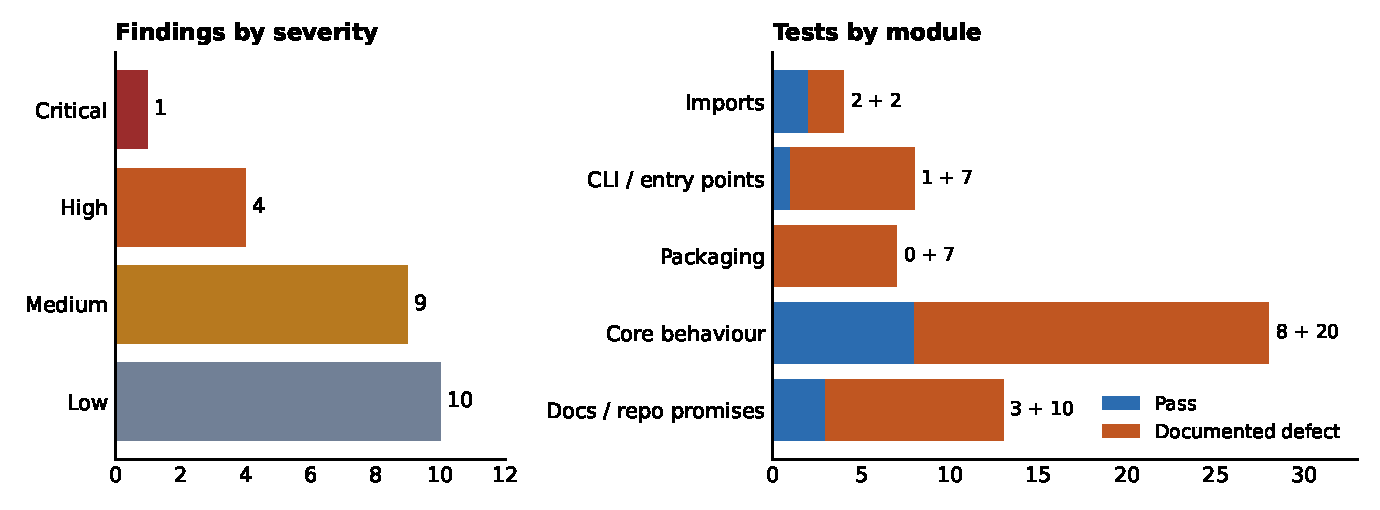
\includegraphics[width=\textwidth]{generated/fig_overview.pdf}
\caption{Findings by severity (left) and tests by module (right; pass\,+\,documented defect).}
\end{figure}

\begin{center}\begin{tabular}{@{}lr@{}}
\toprule
\textbf{Severity} & \textbf{Findings}\\
\midrule
Critical & 1 \\
High & 4 \\
Medium & 9 \\
Low & 10 \\
\midrule
\textbf{Total} & \textbf{24}\\
\bottomrule
\end{tabular}
\end{center}

The repository is explicitly a scaffold, so many findings are ``documented but not implemented'' rather than
regressions. They are reported because the README presents them as working, and because the tests will become useful
regression tests as soon as the features are written.

\section{Key findings}
\subsection*{ISSUE-001 (Critical): the core cannot be imported}
\begin{lstlisting}
$ python -c "import osdagbridge.core.utils.units"
ModuleNotFoundError: No module named 'osdagbridge.core.models'
\end{lstlisting}
\code{core/__init__.py} contains \code{from .models import *} and no \code{models} module exists. Importing any
submodule runs the package \code{__init__} first, so every module below \code{osdagbridge.core} fails: I measured
\textbf{67 of 74 modules}; only the top-level package and the CLI/desktop stubs import. In a temporary copy, adding an
empty \code{models.py} made all 74 modules import, so this is a single root cause with a one-line fix.

\subsection*{ISSUE-023 and ISSUE-024 (High, Low): the test-suite cannot catch it}
\begin{lstlisting}
$ pytest -q        # upstream suite, same install
......             # 6 passed
\end{lstlisting}
All seven upstream test files consist of \code{assert True}. The result above is green even though ISSUE-001 makes the
core unusable. In addition, \code{verification_ddcl_cases.py} does not match pytest's \code{test_*.py} pattern, so
only 6 of the 7 files are collected; the benchmark-verification tests would never run even once written.

\subsection*{ISSUE-014 (High): a check that cannot fail}
\code{check_local_buckling()} accepts no arguments and returns \code{True}. A design check that always passes gives false
assurance in structural software. \code{area()} in the same package returns \code{0.0}. The tests call them with
realistic inputs (a plate with $b/t = 1000$ must fail the check) and document the gap.

\subsection*{ISSUE-009 and ISSUE-010 (Medium): no units, no validation}
\begin{lstlisting}
to_si(250.0, 'mm')   ->  250.0        # expected 0.25
validate_project(None) -> True        # accepts anything
\end{lstlisting}
\code{to_si} returns its input unchanged for every unit, and silently accepts unknown units, so a 250~mm dimension would
be treated as 250~m. \code{validate_project} returns \code{True} for \code{None}, an empty project and a negative span.
Both matter before any numerical code is added.

\subsection*{ISSUE-004 (High): the CLI does not work}
\begin{lstlisting}
$ python -m osdagbridge.cli analyze does_not_exist.yaml
osdagbridge CLI (stub)
$ echo $?
0
\end{lstlisting}
No argument is parsed, no error is possible, and there is no \code{report} command or console-script entry point
(ISSUE-003), so the README's \code{osdagbridge analyze project.yaml --solver native} cannot run.

\section{What works}
The suite also records \npass{} passing behaviours so regressions are caught: the package installs on Python 3.13;
the top-level package imports; the CLI module runs and exits cleanly; the IRC:6 entry resolves in the registry and unknown
codes return \code{None}; the missing OpenSees/OspGrillage adapters raise a clear \code{RuntimeError}; the project's
\code{OsdagError} derives from \code{Exception}; the example input is valid YAML; and, with ISSUE-001 isolated, all
74 modules import. Most of these pin down \emph{current stub behaviour}; they are guard-rails, not evidence of finished
features.

\section{Complete register}
\begin{center}\small\begin{longtable}{@{}p{0.9cm}p{1.5cm}p{2.6cm}p{8.2cm}@{}}
\toprule
\textbf{ID} & \textbf{Sev.} & \textbf{Component} & \textbf{Finding}\\
\midrule
\endhead
001 & Critical & core & Every osdagbridge.\allowbreak{}core.\allowbreak{}* import fails: core/\allowbreak{}\_\allowbreak{}\_\allowbreak{}init\_\allowbreak{}\_\allowbreak{}.\allowbreak{}py imports a missing `models` module \\
002 & Low & packaging & pyproject.\allowbreak{}toml declares license file `LICENSE`, but the repository contains `LICENSE.\allowbreak{}txt` \\
003 & Medium & packaging /\allowbreak{} CLI & No console-script entry point, so the documented `osdagbridge .\allowbreak{}.\allowbreak{}.\allowbreak{}` command does not exist \\
004 & High & CLI & CLI is a stub: ignores all arguments, never fails, has no `report` command \\
005 & Medium & desktop & Desktop app cannot be launched as documented; PySide6 is not a declared dependency \\
006 & Low & packaging /\allowbreak{} reports & LaTeX report template is not shipped in the built wheel \\
007 & Medium & codes & Code registry knows only IRC:6-2017; IRC:22-2015 and IRC:24-2010 are listed in README but unavailable \\
008 & High & loads & IRC:6 vehicle loads and Class A vehicle are empty lists \\
009 & Medium & utils & to\_\allowbreak{}si() never converts units and silently accepts unknown units \\
010 & Medium & utils & validate\_\allowbreak{}project() returns True for every input, including None, \{\} and negative span \\
011 & Medium & plate\_\allowbreak{}girder & PlateGirderDTO has a single field (`name`); no span, width, loading or section data \\
012 & Medium & plate\_\allowbreak{}girder & preliminary\_\allowbreak{}sizing() returns the girder name as `depth\_\allowbreak{}m` \\
013 & Medium & plate\_\allowbreak{}girder /\allowbreak{} solvers & design(), analyse() and run\_\allowbreak{}native\_\allowbreak{}analysis() report success for any input; solver errors use RuntimeError \\
014 & High & bridge\_\allowbreak{}components & Girder area() and check\_\allowbreak{}local\_\allowbreak{}buckling() take no inputs; the check always passes \\
015 & Low & packaging & Three different versions: \_\allowbreak{}\_\allowbreak{}version\_\allowbreak{}\_\allowbreak{} = 0.\allowbreak{}0.\allowbreak{}0, pyproject 0.\allowbreak{}1.\allowbreak{}0, setup.\allowbreak{}cfg 0.\allowbreak{}0.\allowbreak{}0 \\
016 & Low & packaging & requires-python >=3.\allowbreak{}9 but classifiers list only Python 3.\allowbreak{}10 and 3.\allowbreak{}11 \\
017 & Low & packaging & Author e-mail domain looks like a typo: `contact-osdag@efossee.\allowbreak{}in` \\
018 & Low & packaging & core/\allowbreak{}bridge\_\allowbreak{}components/\allowbreak{}super\_\allowbreak{}structure/\allowbreak{} has no \_\allowbreak{}\_\allowbreak{}init\_\allowbreak{}\_\allowbreak{}.\allowbreak{}py \\
019 & Medium & CI & README cites .\allowbreak{}github/\allowbreak{}workflows/\allowbreak{}ci.\allowbreak{}yml but the repository has no CI \\
020 & Low & documentation & README paths are wrong: bridge\_\allowbreak{}types/\allowbreak{}, bridge\_\allowbreak{}components/\allowbreak{} and web/\allowbreak{} are not under src/\allowbreak{}osdagbridge/\allowbreak{} \\
021 & Low & documentation & docs/\allowbreak{}architecture.\allowbreak{}md, developer\_\allowbreak{}guide.\allowbreak{}md and user\_\allowbreak{}guide.\allowbreak{}md are one-line placeholders \\
022 & Low & examples & examples/\allowbreak{}plate\_\allowbreak{}girder/\allowbreak{}verification\_\allowbreak{}case\_\allowbreak{}01.\allowbreak{}yaml and \_\allowbreak{}02.\allowbreak{}yaml contain only a comment \\
023 & High & tests & Upstream test suite is `assert True` placeholders, so it passes while the package's core is unimportable \\
024 & Low & tests & tests/\allowbreak{}integration/\allowbreak{}verification\_\allowbreak{}ddcl\_\allowbreak{}cases.\allowbreak{}py is never collected by pytest \\
\bottomrule
\end{longtable}
\end{center}
Full details of every issue are in Appendix~\ref{app:issues} and in \code{issues/ISSUES.md}.

% ------------------------------------------------------------------ 5
\chapter{Validating the Test Suite}\label{ch:validation}
A test suite that is only ever run on the broken code proves little, so I checked three things.

\begin{enumerate}[leftmargin=1.6em,itemsep=0.25em]
\item \textbf{Each expected failure fails for its stated reason.} Running \code{pytest --runxfail} turns all \nxfail{}
  expected failures into real failures; their messages (for example \code{assert 250.0 == 0.25}, or the list of
  placeholder test files) match the issue text.
\item \textbf{Fixes are detected.} In a copy of the repository I added \code{core/models.py}, a \code{LICENSE} file
  and a consistent version. The tests for ISSUE-001, ISSUE-002 and ISSUE-015 became strict unexpected passes and failed
  the build, as intended; every unrelated test was unchanged. (My first attempt to change \code{setup.cfg} used the wrong
  pattern and changed nothing, which the suite correctly also reported as unchanged.)
\item \textbf{Results do not depend on the machine.} While generating this report's numbers I found that the
  wheel-contents test was silently \emph{skipped} in an environment without \code{setuptools}, producing 62 instead of
  63 results. I changed it to build with isolation and made the report script refuse to run if any test is skipped.
  The final counts (\npass{} passed, \nxfail{} xfailed) are identical in a bare virtual environment and in the system
  Python.
\end{enumerate}

% ------------------------------------------------------------------ 6
\chapter{Recommendations}
In priority order:
\begin{enumerate}[leftmargin=1.6em,itemsep=0.25em]
\item \textbf{Fix ISSUE-001} (one line). Until then nothing under \code{osdagbridge.core} can be used or tested.
\item \textbf{Replace the placeholder tests} and rename \code{verification_ddcl_cases.py}. Adopt the tests in this
  project as a starting point, and add the CI workflow (the README already claims one exists; ISSUE-019).
\item \textbf{Make unsafe stubs fail loudly.} Until implemented, \code{check_local_buckling()}, \code{design()} and
  \code{validate_project()} should raise \code{NotImplementedError} rather than return success.
\item \textbf{Implement unit conversion and input validation} (pydantic is already a dependency) before numerical
  work; add boundary-value tests against the IRC/IS tables.
\item \textbf{Make the CLI real}: argument parsing, non-zero exit codes, a \code{[project.scripts]} entry.
\item \textbf{Tidy metadata and docs}: one version, correct license file and author e-mail, README paths, Python
  floor versus classifiers, non-placeholder documentation.
\end{enumerate}

% ------------------------------------------------------------------ 7
\chapter{Limitations and Future Work}
\begin{itemize}[leftmargin=1.4em,itemsep=0.2em]
\item I audited one commit. The repository is under active development and results may change.
\item The PySide6 desktop GUI, the Django/React web application and the OpenSeesPy, OspGrillage and pythonOCC
  integrations were not exercised, because the audited commit only contains stubs for them. The suite records that fact
  rather than testing them.
\item Severity ratings are my judgement against the scale in Chapter~3.
\item Future work: port the tests into the upstream repository as the features land; add property-based tests for unit
  conversion; add GUI smoke tests (\code{pytest-qt}) and API tests once the web backend exists; verify against the DDCL
  benchmark cases when they are provided.
\end{itemize}

% ------------------------------------------------------------------ 8
\chapter{Conclusion}
The most valuable finding is also the cheapest to fix: a one-line import error that makes 67 of 74 modules unusable,
hidden by a test-suite that cannot fail. The deliverable is not just a list of bugs but a reusable safety net: \ntests{}
traceable tests that stay green now, turn red when a bug is fixed, and become the regression suite for the features
still to be written.

% ------------------------------------------------------------------ appendices
\appendix
\chapter{Issue Register (details)}\label{app:issues}
\small
\subsection*{ISSUE-001: Every osdagbridge.\allowbreak{}core.\allowbreak{}* import fails: core/\allowbreak{}\_\allowbreak{}\_\allowbreak{}init\_\allowbreak{}\_\allowbreak{}.\allowbreak{}py imports a missing `models` module}
\textbf{Severity:} Critical\quad \textbf{Component:} core\par
\textbf{Steps to reproduce.} 1.\allowbreak{} pip install -e .\allowbreak{} 2.\allowbreak{} python -c "import osdagbridge.\allowbreak{}core.\allowbreak{}utils.\allowbreak{}units"\par
\textbf{Expected.} The module imports.\allowbreak{}\par
\textbf{Actual.} ModuleNotFoundError: No module named 'osdagbridge.\allowbreak{}core.\allowbreak{}models'.\allowbreak{} Because core/\allowbreak{}\_\allowbreak{}\_\allowbreak{}init\_\allowbreak{}\_\allowbreak{}.\allowbreak{}py runs `from .\allowbreak{}models import *`, 67 of the package's 74 modules are unimportable (everything under osdagbridge.\allowbreak{}core: utils, solvers, bridge\_\allowbreak{}types, loads, reports, components).\allowbreak{} Only the top-level package and the CLI/\allowbreak{}desktop stubs still import.\allowbreak{}\par
\textbf{Covered by.} test\_\allowbreak{}01\_\allowbreak{}imports.\allowbreak{}py::\allowbreak{}test\_\allowbreak{}core\_\allowbreak{}package\_\allowbreak{}imports, ::\allowbreak{}test\_\allowbreak{}every\_\allowbreak{}module\_\allowbreak{}is\_\allowbreak{}importable (xfail); ::\allowbreak{}test\_\allowbreak{}issue\_\allowbreak{}001\_\allowbreak{}root\_\allowbreak{}cause\_\allowbreak{}is\_\allowbreak{}the\_\allowbreak{}missing\_\allowbreak{}models\_\allowbreak{}module (passes)\par
\textbf{Suggested fix.} Remove the star-import or add core/\allowbreak{}models.\allowbreak{}py.\allowbreak{} With an empty models.\allowbreak{}py all modules import, confirmed in a temporary copy.\allowbreak{}

\subsection*{ISSUE-002: pyproject.\allowbreak{}toml declares license file `LICENSE`, but the repository contains `LICENSE.\allowbreak{}txt`}
\textbf{Severity:} Low\quad \textbf{Component:} packaging\par
\textbf{Steps to reproduce.} pip wheel --no-deps .\allowbreak{}\par
\textbf{Expected.} Build completes without license warnings.\allowbreak{}\par
\textbf{Actual.} BuildBackendWarning: File '.\allowbreak{}.\allowbreak{}.\allowbreak{}/\allowbreak{}LICENSE' cannot be found.\allowbreak{} Also reported: `project.\allowbreak{}license` as a TOML table and License classifiers are deprecated (setuptools will stop accepting them in 2027).\allowbreak{}\par
\textbf{Covered by.} test\_\allowbreak{}03\_\allowbreak{}packaging.\allowbreak{}py::\allowbreak{}test\_\allowbreak{}pyproject\_\allowbreak{}license\_\allowbreak{}file\_\allowbreak{}exists\par
\textbf{Suggested fix.} Rename the file or point to LICENSE.\allowbreak{}txt; migrate to `license = "MIT"` and `license-files`.\allowbreak{}

\subsection*{ISSUE-003: No console-script entry point, so the documented `osdagbridge .\allowbreak{}.\allowbreak{}.\allowbreak{}` command does not exist}
\textbf{Severity:} Medium\quad \textbf{Component:} packaging /\allowbreak{} CLI\par
\textbf{Steps to reproduce.} 1.\allowbreak{} pip install -e .\allowbreak{} 2.\allowbreak{} osdagbridge --help\par
\textbf{Expected.} README documents `osdagbridge analyze project.\allowbreak{}yaml --solver native`.\allowbreak{}\par
\textbf{Actual.} Command not found: pyproject.\allowbreak{}toml has no [project.\allowbreak{}scripts]; the built wheel has no entry\_\allowbreak{}points.\allowbreak{}txt.\allowbreak{}\par
\textbf{Covered by.} test\_\allowbreak{}02\_\allowbreak{}cli.\allowbreak{}py::\allowbreak{}test\_\allowbreak{}console\_\allowbreak{}script\_\allowbreak{}is\_\allowbreak{}declared\par
\textbf{Suggested fix.} Add `[project.\allowbreak{}scripts] osdagbridge = "osdagbridge.\allowbreak{}cli.\allowbreak{}\_\allowbreak{}\_\allowbreak{}main\_\allowbreak{}\_\allowbreak{}:main"` once the CLI parses arguments.\allowbreak{}

\subsection*{ISSUE-004: CLI is a stub: ignores all arguments, never fails, has no `report` command}
\textbf{Severity:} High\quad \textbf{Component:} CLI\par
\textbf{Steps to reproduce.} 1.\allowbreak{} python -m osdagbridge.\allowbreak{}cli analyze does\_\allowbreak{}not\_\allowbreak{}exist.\allowbreak{}yaml --solver native 2.\allowbreak{} echo \$?\par
\textbf{Expected.} An error for the missing file and a non-zero exit status; `--help` lists `analyze` and `report`.\allowbreak{}\par
\textbf{Actual.} Prints `osdagbridge CLI (stub)` and exits 0 for every input, including unknown sub-commands.\allowbreak{}\par
\textbf{Covered by.} test\_\allowbreak{}02\_\allowbreak{}cli.\allowbreak{}py (4 xfail tests: help, acknowledge file, missing file, unknown command)\par
\textbf{Suggested fix.} Implement argparse/\allowbreak{}click sub-commands and return non-zero exit codes on error.\allowbreak{}

\subsection*{ISSUE-005: Desktop app cannot be launched as documented; PySide6 is not a declared dependency}
\textbf{Severity:} Medium\quad \textbf{Component:} desktop\par
\textbf{Steps to reproduce.} python -m osdagbridge.\allowbreak{}desktop\par
\textbf{Expected.} Starts the desktop UI (README).\allowbreak{}\par
\textbf{Actual.} `No module named osdagbridge.\allowbreak{}desktop.\allowbreak{}\_\allowbreak{}\_\allowbreak{}main\_\allowbreak{}\_\allowbreak{}; 'osdagbridge.\allowbreak{}desktop' is a package and cannot be directly executed`.\allowbreak{} README says the GUI uses PySide6, but no optional-dependency group lists it.\allowbreak{} desktop/\allowbreak{}main.\allowbreak{}py only defines `start()` which prints a message.\allowbreak{}\par
\textbf{Covered by.} test\_\allowbreak{}02\_\allowbreak{}cli.\allowbreak{}py::\allowbreak{}test\_\allowbreak{}desktop\_\allowbreak{}package\_\allowbreak{}is\_\allowbreak{}runnable\_\allowbreak{}with\_\allowbreak{}dash\_\allowbreak{}m, ::\allowbreak{}test\_\allowbreak{}pyside6\_\allowbreak{}is\_\allowbreak{}declared\_\allowbreak{}as\_\allowbreak{}a\_\allowbreak{}dependency\par
\textbf{Suggested fix.} Add desktop/\allowbreak{}\_\allowbreak{}\_\allowbreak{}main\_\allowbreak{}\_\allowbreak{}.\allowbreak{}py calling start(); add a `desktop = ["PySide6"]` extra.\allowbreak{}

\subsection*{ISSUE-006: LaTeX report template is not shipped in the built wheel}
\textbf{Severity:} Low\quad \textbf{Component:} packaging /\allowbreak{} reports\par
\textbf{Steps to reproduce.} Build a wheel and list its contents.\allowbreak{}\par
\textbf{Expected.} core/\allowbreak{}reports/\allowbreak{}templates/\allowbreak{}default\_\allowbreak{}template.\allowbreak{}tex is included.\allowbreak{}\par
\textbf{Actual.} Not included: no package-data /\allowbreak{} MANIFEST configuration, and the templates directory is not a package.\allowbreak{}\par
\textbf{Covered by.} test\_\allowbreak{}03\_\allowbreak{}packaging.\allowbreak{}py::\allowbreak{}test\_\allowbreak{}report\_\allowbreak{}templates\_\allowbreak{}are\_\allowbreak{}shipped\_\allowbreak{}in\_\allowbreak{}the\_\allowbreak{}wheel\par
\textbf{Suggested fix.} Declare `[tool.\allowbreak{}setuptools.\allowbreak{}package-data]` for `*.\allowbreak{}tex`.\allowbreak{}

\subsection*{ISSUE-007: Code registry knows only IRC:6-2017; IRC:22-2015 and IRC:24-2010 are listed in README but unavailable}
\textbf{Severity:} Medium\quad \textbf{Component:} codes\par
\textbf{Steps to reproduce.} get\_\allowbreak{}code('IRC:22-2015')\par
\textbf{Expected.} Returns the code module (README: `Included under core/\allowbreak{}utils/\allowbreak{}codes/\allowbreak{}`).\allowbreak{}\par
\textbf{Actual.} Returns None.\allowbreak{} irc22\_\allowbreak{}2015.\allowbreak{}py and irc24\_\allowbreak{}2010.\allowbreak{}py contain only a docstring.\allowbreak{}\par
\textbf{Covered by.} test\_\allowbreak{}04\_\allowbreak{}core\_\allowbreak{}behaviour.\allowbreak{}py::\allowbreak{}test\_\allowbreak{}registry\_\allowbreak{}contains\_\allowbreak{}all\_\allowbreak{}documented\_\allowbreak{}codes (2 params)\par
\textbf{Suggested fix.} Register the modules once implemented, or mark them 'planned' in README.\allowbreak{}

\subsection*{ISSUE-008: IRC:6 vehicle loads and Class A vehicle are empty lists}
\textbf{Severity:} High\quad \textbf{Component:} loads\par
\textbf{Steps to reproduce.} get\_\allowbreak{}vehicle\_\allowbreak{}loads(); class\_\allowbreak{}a()\par
\textbf{Expected.} Axle loads and spacings per IRC:6-2017.\allowbreak{}\par
\textbf{Actual.} Both return [].\allowbreak{} Any analysis built on them would run with no live load.\allowbreak{}\par
\textbf{Covered by.} test\_\allowbreak{}04\_\allowbreak{}core\_\allowbreak{}behaviour.\allowbreak{}py::\allowbreak{}test\_\allowbreak{}irc6\_\allowbreak{}defines\_\allowbreak{}vehicle\_\allowbreak{}loads, ::\allowbreak{}test\_\allowbreak{}class\_\allowbreak{}a\_\allowbreak{}vehicle\_\allowbreak{}has\_\allowbreak{}axles\par
\textbf{Suggested fix.} Implement the load models with unit tests against IRC:6 tables.\allowbreak{}

\subsection*{ISSUE-009: to\_\allowbreak{}si() never converts units and silently accepts unknown units}
\textbf{Severity:} Medium\quad \textbf{Component:} utils\par
\textbf{Steps to reproduce.} to\_\allowbreak{}si(250.\allowbreak{}0, 'mm'); to\_\allowbreak{}si(1.\allowbreak{}0, 'furlong')\par
\textbf{Expected.} 0.\allowbreak{}25 for mm to m; an error for an unknown unit.\allowbreak{}\par
\textbf{Actual.} Returns the input unchanged (250.\allowbreak{}0) in every case.\allowbreak{} A 250 mm value would be treated as 250 m.\allowbreak{}\par
\textbf{Covered by.} test\_\allowbreak{}04\_\allowbreak{}core\_\allowbreak{}behaviour.\allowbreak{}py::\allowbreak{}test\_\allowbreak{}to\_\allowbreak{}si\_\allowbreak{}converts\_\allowbreak{}units (3 params), ::\allowbreak{}test\_\allowbreak{}to\_\allowbreak{}si\_\allowbreak{}rejects\_\allowbreak{}unknown\_\allowbreak{}unit\par
\textbf{Suggested fix.} Implement a unit table and raise OsdagError on unknown units.\allowbreak{}

\subsection*{ISSUE-010: validate\_\allowbreak{}project() returns True for every input, including None, \{\} and negative span}
\textbf{Severity:} Medium\quad \textbf{Component:} utils\par
\textbf{Steps to reproduce.} validate\_\allowbreak{}project(None); validate\_\allowbreak{}project(\{'project': \{'span\_\allowbreak{}m': -5.\allowbreak{}0\}\})\par
\textbf{Expected.} Invalid projects are rejected.\allowbreak{}\par
\textbf{Actual.} Always True.\allowbreak{}\par
\textbf{Covered by.} test\_\allowbreak{}04\_\allowbreak{}core\_\allowbreak{}behaviour.\allowbreak{}py::\allowbreak{}test\_\allowbreak{}validate\_\allowbreak{}project\_\allowbreak{}rejects\_\allowbreak{}invalid\_\allowbreak{}input (4 params)\par
\textbf{Suggested fix.} Validate with pydantic (already a declared dependency) and raise OsdagError.\allowbreak{}

\subsection*{ISSUE-011: PlateGirderDTO has a single field (`name`); no span, width, loading or section data}
\textbf{Severity:} Medium\quad \textbf{Component:} plate\_\allowbreak{}girder\par
\textbf{Steps to reproduce.} dataclasses.\allowbreak{}fields(PlateGirderDTO)\par
\textbf{Expected.} An input schema able to represent examples/\allowbreak{}plate\_\allowbreak{}girder/\allowbreak{}example\_\allowbreak{}basic.\allowbreak{}yaml (span\_\allowbreak{}m: 30.\allowbreak{}0).\allowbreak{}\par
\textbf{Actual.} Only `name: str`.\allowbreak{}\par
\textbf{Covered by.} test\_\allowbreak{}04\_\allowbreak{}core\_\allowbreak{}behaviour.\allowbreak{}py::\allowbreak{}test\_\allowbreak{}dto\_\allowbreak{}models\_\allowbreak{}basic\_\allowbreak{}geometry\par
\textbf{Suggested fix.} Model the YAML schema (pydantic) and load it from file.\allowbreak{}

\subsection*{ISSUE-012: preliminary\_\allowbreak{}sizing() returns the girder name as `depth\_\allowbreak{}m`}
\textbf{Severity:} Medium\quad \textbf{Component:} plate\_\allowbreak{}girder\par
\textbf{Steps to reproduce.} preliminary\_\allowbreak{}sizing(PlateGirderDTO(name='demo'))\par
\textbf{Expected.} A numeric depth in metres.\allowbreak{}\par
\textbf{Actual.} \{'depth\_\allowbreak{}m': 'demo'\}: a string where a length is expected; downstream arithmetic would raise or mislead.\allowbreak{}\par
\textbf{Covered by.} test\_\allowbreak{}04\_\allowbreak{}core\_\allowbreak{}behaviour.\allowbreak{}py::\allowbreak{}test\_\allowbreak{}preliminary\_\allowbreak{}sizing\_\allowbreak{}depth\_\allowbreak{}is\_\allowbreak{}numeric\par
\textbf{Suggested fix.} Compute depth from span (e.\allowbreak{}g.\allowbreak{} span/\allowbreak{}L-over-d ratio) and return a float.\allowbreak{}

\subsection*{ISSUE-013: design(), analyse() and run\_\allowbreak{}native\_\allowbreak{}analysis() report success for any input; solver errors use RuntimeError}
\textbf{Severity:} Medium\quad \textbf{Component:} plate\_\allowbreak{}girder /\allowbreak{} solvers\par
\textbf{Steps to reproduce.} design(None); analyse(object(), solver='no-such-solver'); run\_\allowbreak{}native\_\allowbreak{}analysis(None)\par
\textbf{Expected.} Invalid input or an unknown solver is rejected with an OsdagError.\allowbreak{}\par
\textbf{Actual.} Each returns an 'ok' result.\allowbreak{} The OpenSees/\allowbreak{}OspGrillage adapters raise a bare RuntimeError instead of the project's own OsdagError.\allowbreak{}\par
\textbf{Covered by.} test\_\allowbreak{}04\_\allowbreak{}core\_\allowbreak{}behaviour.\allowbreak{}py::\allowbreak{}test\_\allowbreak{}design\_\allowbreak{}rejects\_\allowbreak{}garbage\_\allowbreak{}input, ::\allowbreak{}test\_\allowbreak{}analyse\_\allowbreak{}rejects\_\allowbreak{}unknown\_\allowbreak{}solver, ::\allowbreak{}test\_\allowbreak{}native\_\allowbreak{}solver\_\allowbreak{}rejects\_\allowbreak{}null\_\allowbreak{}model, ::\allowbreak{}test\_\allowbreak{}adapters\_\allowbreak{}use\_\allowbreak{}project\_\allowbreak{}exception\_\allowbreak{}type\par
\textbf{Suggested fix.} Validate inputs, dispatch on the solver name, derive adapter errors from OsdagError.\allowbreak{}

\subsection*{ISSUE-014: Girder area() and check\_\allowbreak{}local\_\allowbreak{}buckling() take no inputs; the check always passes}
\textbf{Severity:} High\quad \textbf{Component:} bridge\_\allowbreak{}components\par
\textbf{Steps to reproduce.} check\_\allowbreak{}local\_\allowbreak{}buckling(b=1.\allowbreak{}0, t=0.\allowbreak{}001, fy=250.\allowbreak{}0)\par
\textbf{Expected.} An absurdly slender plate (b/\allowbreak{}t = 1000) fails the check; area() derives from the section.\allowbreak{}\par
\textbf{Actual.} TypeError: unexpected keyword argument (no parameters at all).\allowbreak{} With no arguments the check returns True and area() returns 0.\allowbreak{}0, so a structural check that cannot fail would give false assurance.\allowbreak{}\par
\textbf{Covered by.} test\_\allowbreak{}04\_\allowbreak{}core\_\allowbreak{}behaviour.\allowbreak{}py::\allowbreak{}test\_\allowbreak{}girder\_\allowbreak{}area\_\allowbreak{}computes\_\allowbreak{}from\_\allowbreak{}section, ::\allowbreak{}test\_\allowbreak{}local\_\allowbreak{}buckling\_\allowbreak{}check\_\allowbreak{}uses\_\allowbreak{}section\par
\textbf{Suggested fix.} Implement per IS 800 /\allowbreak{} IRC:24 limits and add boundary-value tests.\allowbreak{}

\subsection*{ISSUE-015: Three different versions: \_\allowbreak{}\_\allowbreak{}version\_\allowbreak{}\_\allowbreak{} = 0.\allowbreak{}0.\allowbreak{}0, pyproject 0.\allowbreak{}1.\allowbreak{}0, setup.\allowbreak{}cfg 0.\allowbreak{}0.\allowbreak{}0}
\textbf{Severity:} Low\quad \textbf{Component:} packaging\par
\textbf{Steps to reproduce.} python -c "import osdagbridge, importlib.\allowbreak{}metadata as m; print(osdagbridge.\allowbreak{}\_\allowbreak{}\_\allowbreak{}version\_\allowbreak{}\_\allowbreak{}, m.\allowbreak{}version('osdagbridge'))"\par
\textbf{Expected.} One version everywhere.\allowbreak{}\par
\textbf{Actual.} Prints `0.\allowbreak{}0.\allowbreak{}0 0.\allowbreak{}1.\allowbreak{}0`.\allowbreak{}\par
\textbf{Covered by.} test\_\allowbreak{}03\_\allowbreak{}packaging.\allowbreak{}py::\allowbreak{}test\_\allowbreak{}version\_\allowbreak{}is\_\allowbreak{}single\_\allowbreak{}sourced, ::\allowbreak{}test\_\allowbreak{}setup\_\allowbreak{}cfg\_\allowbreak{}version\_\allowbreak{}matches\_\allowbreak{}pyproject\par
\textbf{Suggested fix.} Single-source the version (dynamic = ["version"]) and delete setup.\allowbreak{}cfg.\allowbreak{}

\subsection*{ISSUE-016: requires-python >=3.\allowbreak{}9 but classifiers list only Python 3.\allowbreak{}10 and 3.\allowbreak{}11}
\textbf{Severity:} Low\quad \textbf{Component:} packaging\par
\textbf{Steps to reproduce.} Read pyproject.\allowbreak{}toml.\allowbreak{}\par
\textbf{Expected.} Declared floor equals the oldest tested version.\allowbreak{}\par
\textbf{Actual.} Floor 3.\allowbreak{}9 versus oldest classifier 3.\allowbreak{}10; 3.\allowbreak{}12+ not classified (install succeeded on 3.\allowbreak{}13).\allowbreak{}\par
\textbf{Covered by.} test\_\allowbreak{}03\_\allowbreak{}packaging.\allowbreak{}py::\allowbreak{}test\_\allowbreak{}requires\_\allowbreak{}python\_\allowbreak{}matches\_\allowbreak{}classifiers\par
\textbf{Suggested fix.} Align requires-python, classifiers, ruff/\allowbreak{}mypy targets, and add a CI matrix.\allowbreak{}

\subsection*{ISSUE-017: Author e-mail domain looks like a typo: `contact-osdag@efossee.\allowbreak{}in`}
\textbf{Severity:} Low\quad \textbf{Component:} packaging\par
\textbf{Steps to reproduce.} Read pyproject.\allowbreak{}toml [project].\allowbreak{}authors.\allowbreak{}\par
\textbf{Expected.} The FOSSEE pages use contact-osdag@fossee.\allowbreak{}in.\allowbreak{}\par
\textbf{Actual.} Domain is efossee.\allowbreak{}in, so mail to the package contact would not reach the team.\allowbreak{}\par
\textbf{Covered by.} test\_\allowbreak{}03\_\allowbreak{}packaging.\allowbreak{}py::\allowbreak{}test\_\allowbreak{}author\_\allowbreak{}email\_\allowbreak{}domain\_\allowbreak{}looks\_\allowbreak{}valid\par
\textbf{Suggested fix.} Correct the address.\allowbreak{}

\subsection*{ISSUE-018: core/\allowbreak{}bridge\_\allowbreak{}components/\allowbreak{}super\_\allowbreak{}structure/\allowbreak{} has no \_\allowbreak{}\_\allowbreak{}init\_\allowbreak{}\_\allowbreak{}.\allowbreak{}py}
\textbf{Severity:} Low\quad \textbf{Component:} packaging\par
\textbf{Steps to reproduce.} List packages for src/\allowbreak{}osdagbridge.\allowbreak{}\par
\textbf{Expected.} Every package directory is a regular package.\allowbreak{}\par
\textbf{Actual.} Implicit namespace package: it works in the wheel, but is inconsistent with every sibling and can be skipped by tools that do not support namespace packages.\allowbreak{}\par
\textbf{Covered by.} test\_\allowbreak{}03\_\allowbreak{}packaging.\allowbreak{}py::\allowbreak{}test\_\allowbreak{}every\_\allowbreak{}package\_\allowbreak{}directory\_\allowbreak{}has\_\allowbreak{}init\par
\textbf{Suggested fix.} Add an \_\allowbreak{}\_\allowbreak{}init\_\allowbreak{}\_\allowbreak{}.\allowbreak{}py.\allowbreak{}

\subsection*{ISSUE-019: README cites .\allowbreak{}github/\allowbreak{}workflows/\allowbreak{}ci.\allowbreak{}yml but the repository has no CI}
\textbf{Severity:} Medium\quad \textbf{Component:} CI\par
\textbf{Steps to reproduce.} ls .\allowbreak{}github\par
\textbf{Expected.} Workflow file exists (README: `Continuous integration runs automatically`).\allowbreak{}\par
\textbf{Actual.} No .\allowbreak{}github directory.\allowbreak{}\par
\textbf{Covered by.} test\_\allowbreak{}05\_\allowbreak{}docs\_\allowbreak{}and\_\allowbreak{}repo.\allowbreak{}py::\allowbreak{}test\_\allowbreak{}ci\_\allowbreak{}workflow\_\allowbreak{}mentioned\_\allowbreak{}in\_\allowbreak{}readme\_\allowbreak{}exists\par
\textbf{Suggested fix.} Add a workflow.\allowbreak{} A ready-made one is in this project: .\allowbreak{}github/\allowbreak{}workflows/\allowbreak{}ci.\allowbreak{}yml.\allowbreak{}

\subsection*{ISSUE-020: README paths are wrong: bridge\_\allowbreak{}types/\allowbreak{}, bridge\_\allowbreak{}components/\allowbreak{} and web/\allowbreak{} are not under src/\allowbreak{}osdagbridge/\allowbreak{}}
\textbf{Severity:} Low\quad \textbf{Component:} documentation\par
\textbf{Steps to reproduce.} Follow README: `python src/\allowbreak{}osdagbridge/\allowbreak{}web/\allowbreak{}backend/\allowbreak{}manage.\allowbreak{}py runserver`.\allowbreak{}\par
\textbf{Expected.} Documented paths exist.\allowbreak{}\par
\textbf{Actual.} Real locations are core/\allowbreak{}bridge\_\allowbreak{}types, core/\allowbreak{}bridge\_\allowbreak{}components and top-level web/\allowbreak{}.\allowbreak{} The runserver command fails with file-not-found; the real manage.\allowbreak{}py is a stub that prints `Django manage stub`.\allowbreak{}\par
\textbf{Covered by.} test\_\allowbreak{}05\_\allowbreak{}docs\_\allowbreak{}and\_\allowbreak{}repo.\allowbreak{}py::\allowbreak{}test\_\allowbreak{}readme\_\allowbreak{}code\_\allowbreak{}locations\_\allowbreak{}exist, ::\allowbreak{}test\_\allowbreak{}readme\_\allowbreak{}runserver\_\allowbreak{}path\_\allowbreak{}exists\par
\textbf{Suggested fix.} Update the README (project-structure tree and Key Code Locations).\allowbreak{}

\subsection*{ISSUE-021: docs/\allowbreak{}architecture.\allowbreak{}md, developer\_\allowbreak{}guide.\allowbreak{}md and user\_\allowbreak{}guide.\allowbreak{}md are one-line placeholders}
\textbf{Severity:} Low\quad \textbf{Component:} documentation\par
\textbf{Steps to reproduce.} cat docs/\allowbreak{}*.\allowbreak{}md\par
\textbf{Expected.} Usable documentation.\allowbreak{}\par
\textbf{Actual.} Each reads 'Documentation placeholder.\allowbreak{}'\par
\textbf{Covered by.} test\_\allowbreak{}05\_\allowbreak{}docs\_\allowbreak{}and\_\allowbreak{}repo.\allowbreak{}py::\allowbreak{}test\_\allowbreak{}docs\_\allowbreak{}are\_\allowbreak{}not\_\allowbreak{}placeholders (3 params)\par
\textbf{Suggested fix.} Write the guides; this report's findings can seed the developer guide.\allowbreak{}

\subsection*{ISSUE-022: examples/\allowbreak{}plate\_\allowbreak{}girder/\allowbreak{}verification\_\allowbreak{}case\_\allowbreak{}01.\allowbreak{}yaml and \_\allowbreak{}02.\allowbreak{}yaml contain only a comment}
\textbf{Severity:} Low\quad \textbf{Component:} examples\par
\textbf{Steps to reproduce.} python -c "import yaml; print(yaml.\allowbreak{}safe\_\allowbreak{}load(open('verification\_\allowbreak{}case\_\allowbreak{}01.\allowbreak{}yaml')))"\par
\textbf{Expected.} Benchmark input data for verification.\allowbreak{}\par
\textbf{Actual.} Parses to None.\allowbreak{}\par
\textbf{Covered by.} test\_\allowbreak{}05\_\allowbreak{}docs\_\allowbreak{}and\_\allowbreak{}repo.\allowbreak{}py::\allowbreak{}test\_\allowbreak{}verification\_\allowbreak{}cases\_\allowbreak{}contain\_\allowbreak{}data (2 params)\par
\textbf{Suggested fix.} Add the DDCL benchmark inputs and expected outputs.\allowbreak{}

\subsection*{ISSUE-023: Upstream test suite is `assert True` placeholders, so it passes while the package's core is unimportable}
\textbf{Severity:} High\quad \textbf{Component:} tests\par
\textbf{Steps to reproduce.} pytest -q in a fresh install\par
\textbf{Expected.} Failing tests when the package is broken.\allowbreak{}\par
\textbf{Actual.} `.\allowbreak{}.\allowbreak{}.\allowbreak{}.\allowbreak{}.\allowbreak{}.\allowbreak{}` all pass, yet ISSUE-001 makes osdagbridge.\allowbreak{}core unusable.\allowbreak{} All 7 test files are placeholders.\allowbreak{}\par
\textbf{Covered by.} test\_\allowbreak{}05\_\allowbreak{}docs\_\allowbreak{}and\_\allowbreak{}repo.\allowbreak{}py::\allowbreak{}test\_\allowbreak{}upstream\_\allowbreak{}tests\_\allowbreak{}contain\_\allowbreak{}real\_\allowbreak{}assertions\par
\textbf{Suggested fix.} Replace the placeholders.\allowbreak{} This project's tests can be ported as a starting point.\allowbreak{}

\subsection*{ISSUE-024: tests/\allowbreak{}integration/\allowbreak{}verification\_\allowbreak{}ddcl\_\allowbreak{}cases.\allowbreak{}py is never collected by pytest}
\textbf{Severity:} Low\quad \textbf{Component:} tests\par
\textbf{Steps to reproduce.} pytest --collect-only -q\par
\textbf{Expected.} 7 test files are collected.\allowbreak{}\par
\textbf{Actual.} 6 are collected; verification\_\allowbreak{}ddcl\_\allowbreak{}cases.\allowbreak{}py does not match the default `test\_\allowbreak{}*.\allowbreak{}py` pattern, so even once filled in, the verification cases would never run.\allowbreak{}\par
\textbf{Covered by.} test\_\allowbreak{}05\_\allowbreak{}docs\_\allowbreak{}and\_\allowbreak{}repo.\allowbreak{}py::\allowbreak{}test\_\allowbreak{}every\_\allowbreak{}upstream\_\allowbreak{}test\_\allowbreak{}file\_\allowbreak{}is\_\allowbreak{}collectable\par
\textbf{Suggested fix.} Rename it to test\_\allowbreak{}verification\_\allowbreak{}ddcl\_\allowbreak{}cases.\allowbreak{}py.\allowbreak{}

\normalsize

\chapter{Reproducing the Results}
\begin{lstlisting}
git clone https://github.com/osdag-admin/OsdagBridge.git OsdagBridge
git -C OsdagBridge checkout 2cb7ddc
pip install -r requirements-test.txt
OSDAGBRIDGE_REPO=./OsdagBridge pytest             # 17 passed, 46 xfailed
OSDAGBRIDGE_REPO=./OsdagBridge pytest --runxfail  # the 46 raw failures
python tools/render_issues.py                     # regenerate ISSUES.md
./demo.sh                                         # paced walkthrough
\end{lstlisting}

\end{document}
